
\section{Related Work}

Many approaches have so far been taken in an attempt to improve a computer's ability to perform the task of finite element meshing. The following subsections present an overview of the research conducted for the various aspects of the project which are more explicitly outlined under ``Aims and Objectives"

\subsection{Traditional Stress refinement methods}

A number of methods exist to perform mesh refinement based on a stress gradient for a mesh, with the most common being higherarchical refinementent also known as h-refinement and relocation refinement or r-refinement\cite{HandPRefinements} \cite{RRefinement}\\ 

\noindent
\textbf{h-refinement: }
H-refinement is the process of recursively refining a mesh by splitting elements into additional sub elements. This process can be performed for elements with both both triangular and quadrilateral shapes. \cite{HandPRefinements}. \\ 

\noindent
\textbf{r-refinement: }
R-refinement is a method which attempts to improve the quality of the stress gradient without the alteration of the mesh element count and thus the computational cost. This is achieved by the relocation of elements within the mesh which effectively increases the size of elements in areas of low stress, while reducing the size in areas where stress is high \cite{RRefinement}.


\subsection{Uses of Artificial Intelligence and Machine Learning}

\noindent
Within the domains of AI and machine learning methods such as neural networks \cite{NeuralNetworks}, case based reasoning \cite{caseBasedReasoning} and inductive logic programming \cite{DolsakPaper94} have all been adopted to facilitate generation of meshes comparable to that of human experts.  Similarly there has also been effort to combine multiple numerical methods simultaneously for solving re meshing problems \cite{TraditionalHybridRefinement} although effort to combine the two approaches does not appear to have so far been made.\\ 

\noindent
Due to the difficulty of obtaining meshes which hold commercial interest the majority of researchers working in this field have had to result to the use of training sets developed within academia \cite{DolsakPaper91}. The primary issue associated with this is that often the training data does not exhibit the level of complexity that you would expect in many industrial sectors. Many researchers must accept this as a limitation or agree commercial terms with an organisation in order to gain access to their models \cite{DittmerMeshQualityMet}.\\ 

\noindent
Having reviewed a variety of different AI based applications to FE the use of Inductive Logic Programming (ILP) used by Bojan Dolsak et al is of greatest interest. ILP is a machine learning method first presented by Stephen Muggleton in his 1991 paper ``Inductive Logic Programming" \cite{MuggletonILP}. Muggleton suggests that the traditional approaches of machine learning which rely on use of extensive data sets and statistical analysis are poor in the case of many real world problems for which data is not available \cite{ILPYoutubeLecture}. Muggleton cites Human learning as an example of use of ILP style techniques where understanding of new concepts is achieved not through crunching large volumes of data points but instead  the use of induction on a relatively concise set of background facts and examples obtained from previous life experiances \cite{ILPYoutubeLecture}. \\ 

\noindent
ILP uses three types of input information in order to hypothesise additional facts about the system. These three types of input information are: \\ 

\begin{itemize}
\item Positive examples  of what constitutes an area that is well meshed
\item Negative example of areas that are poorly meshed
\item Background facts
\end{itemize}

\noindent
Using this information ILP is capable of hypothesising rules by determining which rules can exist within the system where given the set of background facts all positive examples are satisfied while few or none of the negative examples are. Although ILP requires a body of additional metadata associated with each mesh this is easier to obtain making ILP a highly practical solution. Along with his publication Muggletons also released his implementation of an ILP algorithm as a program titled ``Golem" \cite{Golem}, Golem was applied by Dolsak to the problem of mesh refinement with a training set of just five meshes \cite{DolsakPaper94}. The resulting rule set when applied to subsequent models was able to correctly classify and re mesh areas with an average accuracy of 78\% for a range of geometries \cite{DolsakPaper94} \cite{appOfILPToFEMeshDesign}. \\

\noindent
Dolsak's choice of metadata for the ILP method to generate mesh rules is based on the classification of edges within the FE model. Dolsak recognises that edges act as an important intersections within the model and as such provide useful items of reference when designing heruristics with which to reason about the model \cite{DolsakPaper94} \cite{appOfILPToFEMeshDesign}.  For example if it is know that an edge has a force applied close to it based on the initial model conditions then other edges that intersect it should be additionally remeshed meshed \cite{DolsakPaper91} \cite{appOfILPToFEMeshDesign}. \\ 

\noindent
The format of the rules also make them attractive for experimenting with as part of a hybrid method since the method determines how to refine the mesh based on the arrangement of edges. This detail of analysis of the mesh is at a comparable detail to that of a traditional splitting method such as h-refinement which will likely to improve the ease at which the two methods can be combined simultaneously in the latter stages of the project. \\ 

\subsection{Quality metrics}
\noindent
Finally work has also been done on establishing valid metrics for assessing the quality of a mesh automatically \cite{DittmerMeshQualityMet, NeuralNetworks} Metrics for meshes have been research far more extensively that AI methods due to their use for comparing different stress based refinements. There are also cases of common metrics being used for industrial meshing applications \cite{DittmerMeshQualityMet}. Although there are metrics for assessing a mesh on a global level such as element count score the consensus is that due to the variation in meshes this is less reliable than assessing quality based on the properties of individual elements within the mesh \cite{DittmerMeshQualityMet} \\

\begin{figure}
  \centerline{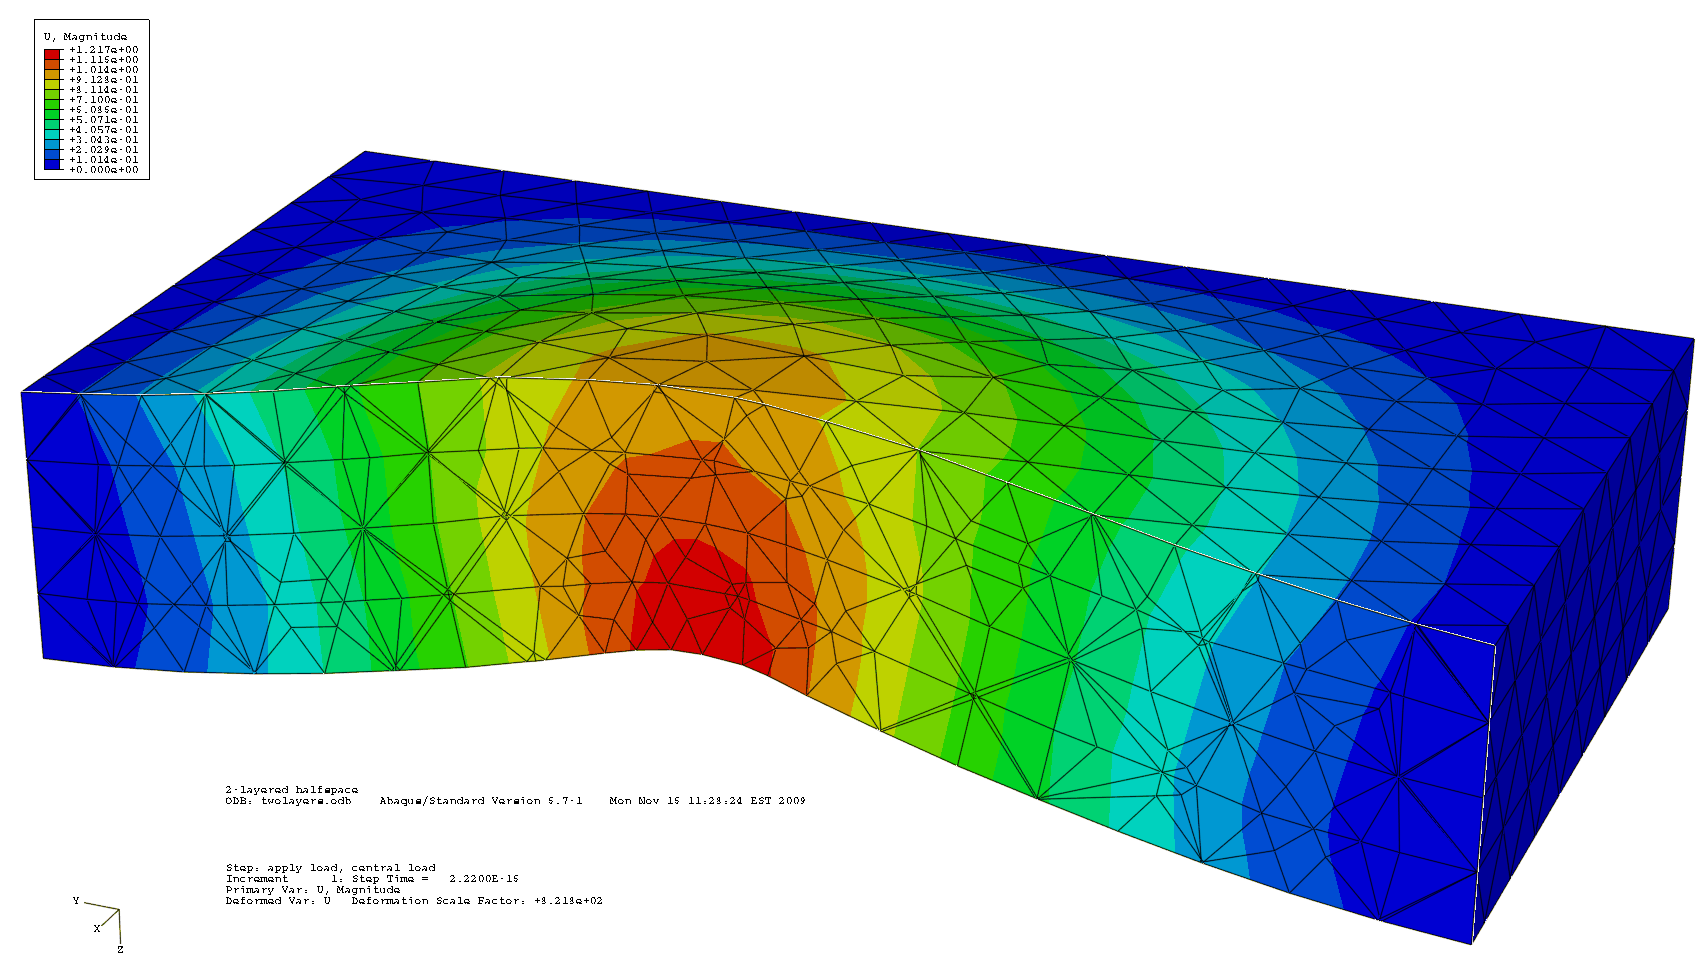
\includegraphics[width=120mm, scale=1]{../Graphics/MeshQualityDeterioration.png}}
  \caption{Example of how elements can be distorted in order to fit a geometry which will result in deterioration of gradient quality (image source: \cite{PoorFEElementShapes})}
\end{figure}


\noindent
Localised metrics associated with the quality of each element have shown to be accurate for predicting the overall quality of a mesh when taking the average for each metric across all elements \cite{DittmerMeshQualityMet}. The quality of an elements shape is important since the stress values which are computed for the area within the element are calculated using the stress values at each of the nodes which enclose it \cite{IntroductionToFE}. Elements are typically deformed near parts of the geometry where its shape simply does not allow a uniform element to be placed, an example of where this has occurred can be seen in figure 2.\\ 

\noindent
Some key shape metrics identified by Dittmer et al include (ideal values are for elements of quadrilateral type as used in  the current prototypes):

\begin{enumerate}[label=\Alph*]
\item Aspect ratio – longest side / shortest side, ideal value is 1
\item Maximum corner angle - widest internal angle to element, ideal is 90\degree
\item Maximum parallel deviation - how skewed the element is, ideal is 0\degree
\end{enumerate}